\input{../../../university/.preambles/01-semester_work}
\input{../../../university/.preambles/10-russian}
\input{../../../university/.preambles/20-math}
\input{../../../university/.preambles/30-physics}
\usepackage{mathrsfs}
\renewcommand{\H}{\mathscr{H}}
\begin{document}
\maketitlepagewithvariant{Автотракторный факультет}{<<Теоретическая механика>>}
{Теоретическая механика}{студент группы Ф-369\\{{ Голубев~А.~В. }}}
{профессор, д.~ф.-м.~н.\\Брискин~Е.~С.}{№2}{{{ 7 }}}

\setcounter{page}{2}

Однородная пластина массой \( m_1 \), геометрические размеры которой известны,
может вращаться вокруг вертикальной оси \( Oz \). С пластиной жестко связана
спиральная пружина жесткостью \( c \). По каналу \( AB \) пластины из точки
\( A \) к точке \( B \) без трения движется точка \( M \) массой \( m_2 \).
Составить дифференциальные уравнения движения системы, используя уравнения
Лагранжа второго рода, уравнения Лагранжа первого рода, уравнения Гамильтона.

\vspace{3em}

\begin{figure}[ht]
    \center
    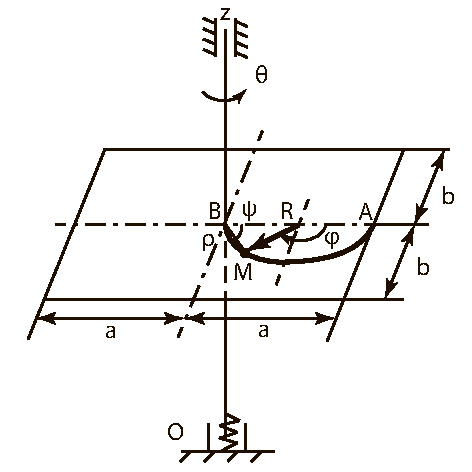
\includegraphics[width=.5\textwidth]{picture}
\end{figure}

\emph{\textbf{Решение:}}

\section{Уравнения Лагранжа второго рода}
    Система имеет две степени свободы. В качестве обобщенных координат выберем
    угол поворота пластины \( q_1 = \theta \) и угол \( q_2 = \phi \).
    
    Составляем уравнения Лагранжа второго рода, которые примут вид:
    \begin{align*}
        & \der{}{t}\left(\pder{L}{\dot{\theta}}\right) - \pder{L}{\theta} = 0, \\
        & \der{}{t}\left(\pder{L}{\dot{\phi}}\right) - \pder{L}{\phi} = 0.
    \end{align*}
    
    Кинетическая энергия системы имеет вид:
    \[
        T = \frac{m_1(a^2 + b^2)}{3}\frac{\dot{\theta}^2}{2} +
        \frac{m_2R^2}{2}\left(\dot{\phi}^2 + 4\dot{\theta}^2\cos^2\frac{\phi}{2}
        + 4\dot{\theta}\dot{\phi}\cos^2\frac{\phi}{2}\right).
    \]
    
    Потенциальная энергия системы определяется потенциальной энергией
    закручивания пружины. В обобщенных координатах она имеет вид:
    \[
        \varPi = \frac{1}{2}c\theta^2.
    \]
    
    Тогда функция Лагранжа системы имеет вид:
    \[
        L = T - \varPi = \frac{m_1(a^2 + b^2)}{3}\frac{\dot{\theta}^2}{2} +
        \frac{m_2R^2}{2}\left(\dot{\phi}^2 + 4\dot{\theta}^2\cos^2\frac{\phi}{2}
        + 4\dot{\theta}\dot{\phi}\cos^2\frac{\phi}{2}\right) - \frac{1}{2}c\theta^2.
    \]
    
    Подставляя в уравнения Лагранжа второго рода, получим:
    \begin{align*}
        & \der{}{t}\left[\frac{m_1(a^2 + b^2)}{3}\dot{\theta} +
        4m_2R^2\dot{\theta}\cos^2\frac{\phi}{2} +
        2m_2R^2\dot{\phi}\cos^2\frac{\phi}{2}\right] + c\theta = 0, \\
        & \der{}{t}\left[m_2R^2\dot{\phi} + 2m_2R^2\dot{\theta}
        \cos^2\frac{\phi}{2}\right] + m_2R^2\dot{\theta}^2\sin\phi +
        m_2R^2\dot{\theta}\dot{\phi}\sin\phi = 0.
    \end{align*}
    
    Тогда система дифференциальных уравнений движения имеет вид:
    \begin{align*}
        & \ddot{\theta}\left[\frac{m_1(a^2 + b^2)}{3} + 4m_2R^2
        \cos^2\frac{\phi}{2}\right] + 2m_2R^2\ddot{\phi}\cos^2\frac{\phi}{2} -
        (2\dot{\theta} + \dot{\phi})\dot{\phi}\sin\phi + c\theta = 0, \\
        & \ddot{\phi} + 2\ddot{\theta}\cos^2\frac{\phi}{2} + \dot{\theta}^2
        \sin\phi = 0.
    \end{align*}

% переписать уравнения под мою систему
    
\section{Уравнения Лагранжа первого рода}
    В качестве обобщённых координат выберем сферические координаты точки
    \( М \) \( \rho, \theta, \phi \). Так как точка находится в
    канале, то имеют место связь \( f_1 = \rho - R\cos\frac{\phi}{2} = 0 \).

    В этих обобщённых координатах кинетическая энергия системы записывается в
    виде
    \[
        T = \frac{m_1}{3}(a^2+b^2)\frac{\dot{\theta^2}}{2} 
        + \frac{m_2 R^2}{2}\dot{\varphi^2} + 2\dot{\theta}\rho^{2} m_2
        + 2\dot{\theta}\dot{\varphi}\rho^2 m_2
    \]
    а потенциальная --
    \[
        \varPi = \frac{1}{2}c\theta^2.
    \]
    Тогда функция Лагранжа системы имеет вид:
    \[
        L = \frac{m_1}{3}(a^2+b^2)\frac{\dot{\theta^2}}{2} 
        + \frac{m_2 R^2}{2}\dot{\varphi^2} + 2\dot{\theta}\rho^2 m_2
        + 2\dot{\theta}\dot{\varphi}\rho^2 m_2 - \frac{1}{2}c\theta^2
    \]

    Для обобщённых коорднат составляем уравнения Лагранжа первого рода:
    \begin{align*}
        & \der{L}{\rho} = -4\dot{\theta}\rho m_2 \left( 1 + \dot{\varphi}\right) 
        = \lambda_1, \\
        & \frac{d}{dt}\left( \frac{m_1}{3}(a^2+b^2)\dot{\theta}
        + 2\rho^{2} m_2 + 2\dot{\varphi}\rho^2 m_2 \right) + c\theta = 0, \\
        & \frac{d}{dt}\left( m_2 R^2 \dot{\varphi} + 2\dot{\theta}\rho^2 m_2 \right) 
        = \lambda_1 \frac{R}{2} \sin\frac{\varphi}{2}.
    \end{align*}

    Выразив из двух последних уравнений \( \lambda_1 \) и
    подставив в первые два уравнения с учётом \( f_1 \), получаем
    знакомые уравнения движения в координатах \( \theta \) и \( \phi \):
    \begin{align*}
        & R^2 \ddot{\varphi} + 2\ddot{\theta}\rho^2 + 4\dot{\theta}\dot{\rho}\rho = 
        - \frac{R}{2}\left( 4\dot{\theta}\rho - 4\dot{\theta}\dot{\varphi}\rho \right)\sin\frac{\varphi}{2}, \\
        & \frac{m_1}{3}(a^2+b^2)\ddot{\theta} + 4\dot{\theta}\rho m_2 + 2\ddot{\varphi}\rho^2 m_2
        + 4\dot{\varphi}\dot{\rho}\rho m_1 + c\theta = 0
    \end{align*}

\section{Уравнения Гамильтона}
    В качестве обобщенных координат выберем угол поворота пластины \( \theta \)
    и угол \(\phi \).
    
    Составляем канонические уравнения Гамильтона, которые примут следующий вид:
    \[
        \dot{p_\theta} = -\pder{H}{\theta},\ \dot{p_\phi} = -\pder{H}{\phi}.
    \]
    
    Определяем обобщенные импульсы. Функция Лагранжа системы выглядит
    следующим образом:
    \[
        L = T - \varPi = \frac{m_1(a^2 + b^2)}{3}\frac{\dot{\theta}^2}{2} +
        \frac{m_2R^2}{2}\left(\dot{\phi}^2 + 4\dot{\theta}^2\cos^2\frac{\phi}{2}
        + 4\dot{\theta}\dot{\phi}\cos^2\frac{\phi}{2}\right) - \frac{1}{2}c\theta^2.
    \]
    Тогда:
    \begin{align*}
        & p_\theta = \pder{L}{\dot{\theta}} = \left[\frac{m_1}{3}(a^2+b^2)
        + 4m_2 R^2 \cos^{2}{\frac{\varphi}{2}}
        - 8\cos^4{\frac{\varphi}{2}}\right]\dot{\theta}
        + 4\frac{p_\varphi}{m_2 R^2}\cos^{2}{\frac{\varphi}{2}}, \\
        & p_\phi = \pder{L}{\dot{\phi}} = m_2 R^2 \varphi^2 
        + 2m_2 R^2\frac{p_\theta - \frac{4p_\varphi}{m_2 R^2}\cos^2{\varphi}{2}}
        {\frac{m_1}{3}(a^2+b^2)+4m_2R^2\cos^2\frac{\varphi}{2}
        - 8\cos^4\frac{\varphi}{2}}.
    \end{align*}
    
    Определяем функцию Гамильтона 
    \begin{align*}
        & \H = p_\theta\dot{\theta} + p_\phi\dot{\phi} - L =
        \frac{p_{\theta^2} - 4f\cos^2\frac{\varphi}{2}}{g}
        + \left(\frac{p^{2}_{\varphi}}{m_2 R^2} 
        - 2\left[\frac{p_\theta p_\varphi - 4cp_\varphi 
        \cos^2\frac{\varphi}{2}}{g}\right] \right) \\
        & - \frac{m_1}{6}(a^2+b^2)\left(\frac{p_\theta 
        - 4f\cos^2\frac{\varphi}{2}}{g}\right)^{2}
        - \frac{m_2 R^2}{2}\left[ c - 2\left( 
        \frac{\rho_{\theta} - 4c\cos^2\frac{\varphi}{2}}{g} 
        \right)\cos^2\frac{\varphi}{2} \right]^2 \\
        & + 4\left( \frac{\rho_\theta - 4c\cos^2\frac{\varphi}{2}}{g} \right)
        + \left( \frac{\rho_\theta - 4c\cos^2\frac{\varphi}{2}}{g} \right)
        \left( c - 2\left[ \left( \frac{\rho_\theta - 4c
        \cos^2\frac{\varphi}{2}}{g} \right) \right]
        \cos^2\frac{\varphi}{2} \right) + \frac{1}{2}c\theta^2
    \end{align*}
    где 
    \begin{align*}
        & g = \frac{m_1}{3}(a^2+b^2)+4m_2R^2\cos^2\frac{\varphi}{2}
        - 8\cos^4\frac{\varphi}{2}, \\
        & f = \frac{p_\varphi p_\theta}{m_2 R^2}, \\
        & c = \frac{p_\varphi}{m_2 R^2}.
    \end{align*}
    
    Тогда, дифференцируя и подставляя в уравнения Гамильтона, получим систему
    дифференциальных уравнений движения:
    \begin{align*}
        & \ddot{\theta}\left[\frac{m_1(a^2 + b^2)}{3} + 4m_2R^2
        \cos^2\frac{\phi}{2}\right] + 2m_2R^2\ddot{\phi}\cos^2\frac{\phi}{2} -
        (2\dot{\theta} + \dot{\phi})\dot{\phi}\sin\phi + c\theta = 0, \\
        & \ddot{\phi} + 2\ddot{\theta}\cos^2\frac{\phi}{2} + \dot{\theta}^2
        \sin\phi = 0.
    \end{align*}
\end{document}